\chapter{Conclusion and future works}
\section{High frequency trading system}
Over the last few decades, information technology, including computing speed and memory volume, has made great development. According to this trend, a new class of trading system, which is called high frequency trading (HFT), has appeared to today's financial markets. Generally speaking,  HFT represents a program trading platform that uses powerful computers to transact a great number of orders at very fast speeds. It becomes more and more popular because of some key factors:\\
\begin{itemize}
\item \textbf{Narrowing Spreads}. In 2001, the unit of quoting prices in U.S. Stock exchanges changed from fractions to decimals. so the minimum spread between the bid and ask prices decreased from 1/6th of a dollar (6.25 cents) to one cent. The change of  price unit provides traders better alternatives to seek spread arbitrages, which results in a strong boost in algorithmic trading system.  \\
\item \textbf{Regulation changes}. In 2005, the Securities and Exchange Commission(SEC) passed the Regulation National Market System(Reg.NMS), which improved transparency and competition among different financial markets. Besides, this regulation also required trade orders to be posted nationally instead of at individual exchanges. So traders can be beneficial of profit from small price difference of a security among different exchanges. \\
\end{itemize}

High frequency trading is an extension case of algorithmic trading, which turns over small positions of a security very frequently. The U.S. Securities and Exchanges Commission conclude specific characteristics of HFT:\\

\begin{itemize}
\item Submit some orders and cancel them soon after the submission.
\item Maintain very few or no overnight positions. 
\item Maintain very short time intervals for specific security positions and turn over very frequently of many small positions in one or more financial tools.
\item Utilize complicated and high performance computing program to generate, execute or cancel orders.
\item Make use of individual data from exchanges and servers that belong to co-location provider in order to minimize network or other types of latencies. 
\end{itemize}

According to recent survey(Anuj Agarwal,2012,\cite{hft_future}), high frequency trading has taken a great number of share in U.S. and European equity trading volume. As shown in figure \ref{fig.1}, in U.S., the percentage of HFT in equity turnover by volume maintained growth trend overall from year 2005 to 2010. For example, in 2010, HFT occupied 56\% by volume of the entire equity turnover, increased from 21 \% in 2005. 

\begin{figure}[hbtp]
  \begin{center}
    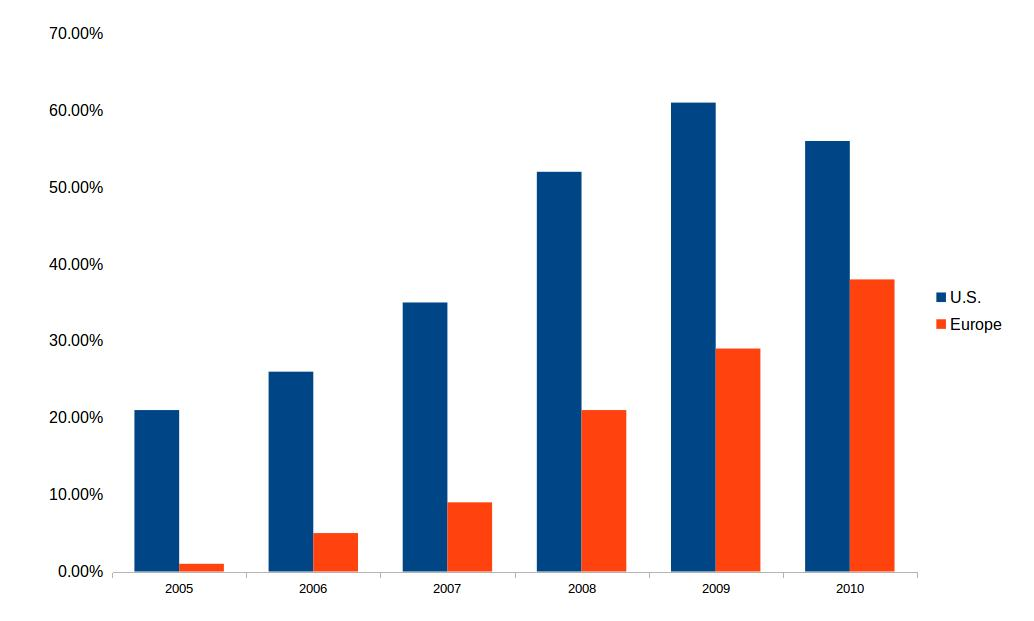
\includegraphics[width=6.5in,height=3.5in]{figures/hft_percentage.jpg}
  \end{center}
\caption{High frequency trading as a \% of equity turnover by volume, U.S. and by value, Europe 2005-2010, x axis represents year and y axis represents percentage of high frequency trading.} \label{fig.1}
\end{figure}

Similar situation happened in Europe. HFT only accounted for 1\% of equity turnover by value in 2005. The percentage surged to 38 \% in 2010, increased from 29 \% just a year ago.

\section{Limit order book dynamics}

\section{Purpose of the dissertation}